\section{Concepts of work, energy and power}
	Before examining the work-energy theorem and conservation laws in mechanics, we must establish rigorous vector definitions for the foundational quantities of work, energy, and power:
	\begin{itemize}
		\item \emph{Work:} an activity where a force acting on a system causes a displacement.
		
		\item \emph{Energy:} the capacity of a system for doing work. A system may possess energy in the form of motion or position.
		
		\item \emph{Kinetic energy:} the energy possessed by a system by virtue of its motion.
		
		\item \emph{Potential energy:} the energy possessed by a system by virtue of its position or configuration.
		
		%\item \emph{Conservative force:} %a force whose total work done on a particle depends only on the initial and final positions, and is completely independent of the path taken.
		
		%\item \emph{Non-conservative force:} %a force whose work done along a path depends on the specific trajectory taken, leading to mechanical energy dissipation (e.g., friction, fluid drag).
		
		\item \emph{Power:} the rate at which work is done or energy is used by a system.
	\end{itemize}

	\subsection{Work}
		Let us consider a particle of mass $m$ which is moving on an arbitrary path between points $A$ and $B$. Suppose when the particle is at point $P$ with a position vector $\vb{r}$, it is under the influence of some force $\vb{F}$ which causes it to get displaced to another point $Q$ with a position vector $\vb{r}+\dd{\vb{r}}$.
		\begin{figure}[h!]
			\centering
			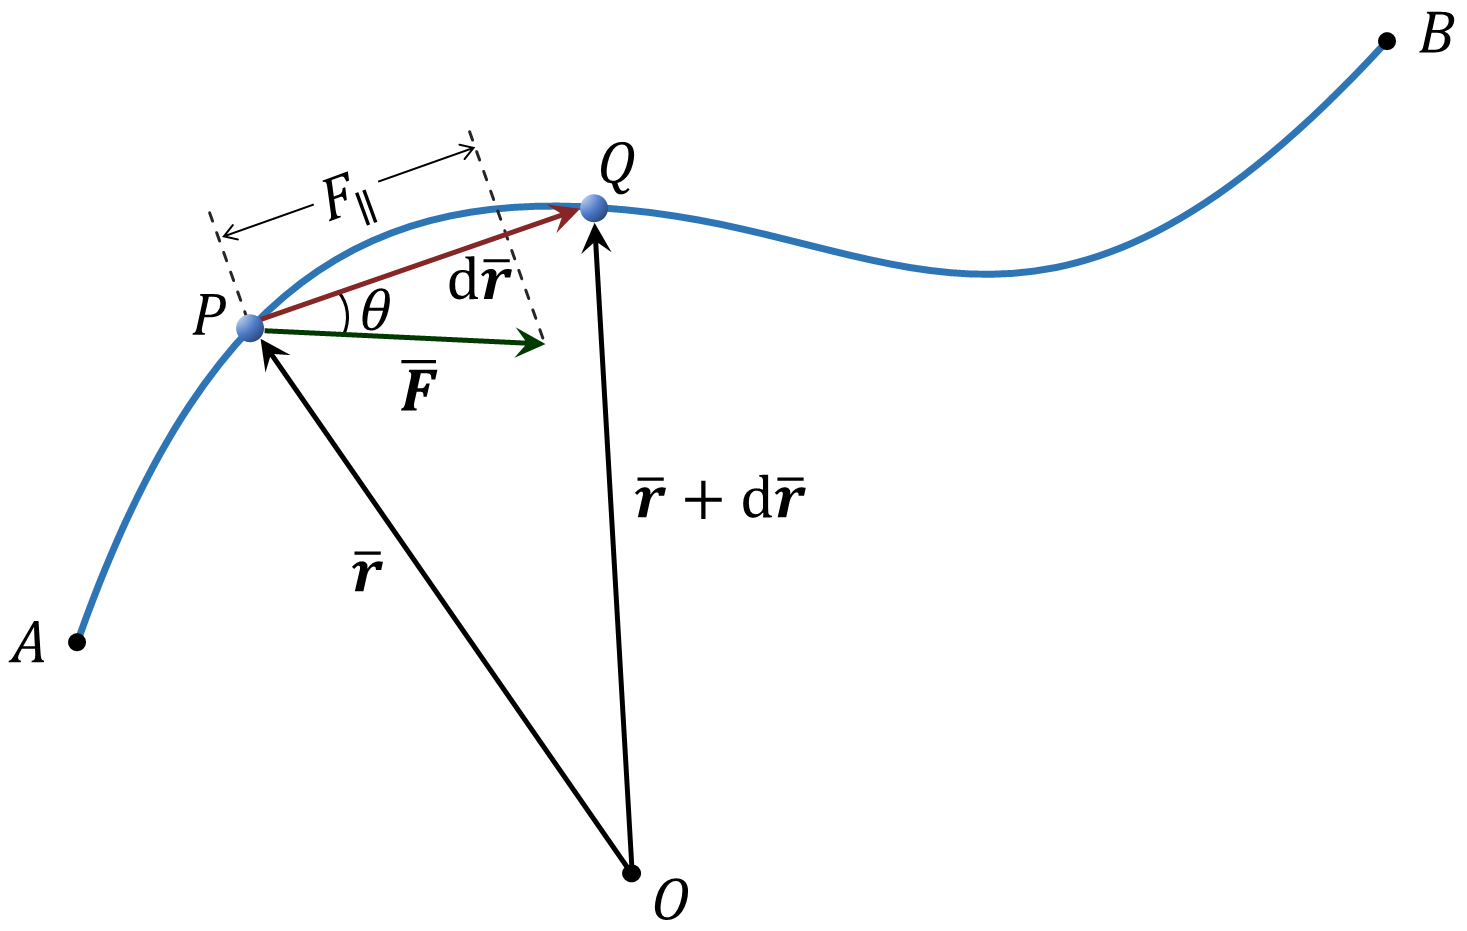
\includegraphics[width=0.6\textwidth]{figures/fig_work-concept.png}
		\end{figure}
		
		The infinitessimal amount of work done by the force $\vb{F}$ in moving the particle from $P$ to $Q$ is
		\begin{align*}
			\dd{W}=\vb{F}\cdot\dd{\vb{r}}=F\cos{\theta}\dd{r}=F_\parallel\dd{r}
		\end{align*}
		where $\theta$ is the angle between $\vb{F}$ and $\dd{\vb{r}}$ and $F_\parallel=F\cos{\theta}$ is the projection of $\vb{F}$ along $\dd{\vb{r}}$.
		
		Hence, the total work done by the force $\vb{F}$ in moving the particle from $A$ to $B$ is
		\begin{align*}
			W&=\int\limits_{A}^{B}{\dd{W}}=\int\limits_{A}^{B}{\vb{F}\cdot\dd{\vb{r}}}=\int\limits_{A}^{B}{F\cos{\theta}\dd{r}}
		\end{align*}
	
	\subsection{Energy}
	
	\subsection{Power}